% !TEX root = ../my-thesis.tex
%
\chapter{Introduction}
\label{sec:intro}

\cleanchapterquote{You can't do better design with a computer, but you can speed up your work enormously.}{Wim Crouwel}{(Graphic designer and typographer)}

% ---------------------------------------
\section{From seven sisters to a powerhouse of astronomy}




% ---------------------------------------
\section{An observational history of open clusters}

\blindtext

% Plot of catalogues of OCs
\begin{figure}[htb]
	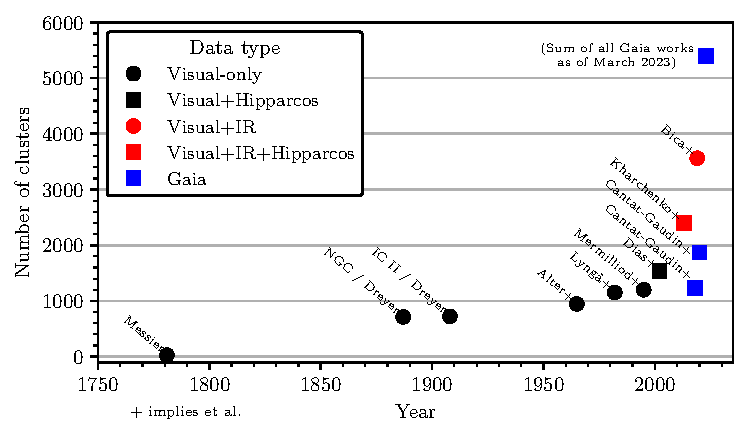
\includegraphics[width=\textwidth]{fig/c1/catalogues.pdf}
	\caption{TODO}
	\label{fig:intro:catalogues}
\end{figure}


% Plot of reported OCs
\begin{figure}[htb]
	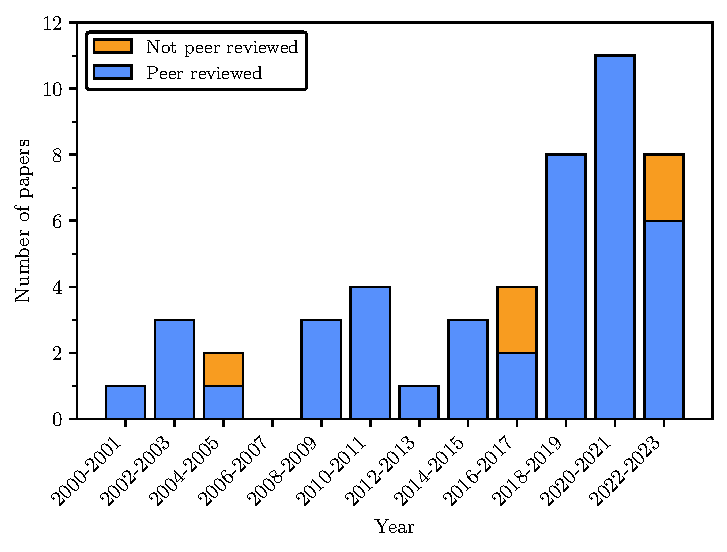
\includegraphics[width=\textwidth]{fig/c1/papers.pdf}
	\caption{TODO}
	\label{fig:intro:papers}
\end{figure}


% ---------------------------------------
\section{Open clusters in the \gaia\ era}


% ---------------------------------------
\section{The theoretical background of star clusters}


% ---------------------------------------
\section{Thesis structure}
\label{sec:intro:structure}

\textbf{Chapter \ref{sec:intro}} \\[0.2em]
\blindtext

\textbf{Chapter \ref{sec:intro}} \\[0.2em]
\blindtext

\textbf{Chapter \ref{sec:intro}} \\[0.2em]
\blindtext

\textbf{Chapter \ref{sec:intro}} \\[0.2em]
\blindtext

\textbf{Chapter \ref{sec:intro}} \\[0.2em]
\blindtext
